\documentclass[11pt]{extarticle}
\usepackage{manualdoprofessor}
\usepackage{fichatecnica}
\usepackage{lipsum,media9}
\usepackage[justification=raggedright]{caption}
\usepackage[one]{bncc}
\usepackage[werner]{../edlab}
\usepackage{marginnote}
\usepackage{pdfpages}
\usepackage[printwatermark]{xwatermark}
%\newwatermark[pagex=2]{\includegraphics{testc.png}}
%\newwatermark[oddpages]{\includegraphics{test.png}}
%\newwatermark[evenpages]{\includegraphics{testb.png}}

\pagecolor{cyan!0!magenta!10!yellow!28!black!28!}

\newcommand{\AutorLivro}{Ademir Barbosa Júnior}
\newcommand{\TituloLivro}{O sapo voador}
\newcommand{\Tema}{Aventuras em contextos imaginários ou realistas; urbanos; rurais; locais; internacionais}
\newcommand{\Genero}{Poemas; trava-línguas; parlendas; adivinhas; provérbios; quadrinhas; etc}
%\newcommand{\imagemCapa}{./images/PNLD0001-01.png}
\newcommand{\issnppub}{978-65-99583-60-5}
\newcommand{\issnepub}{978-65-99583-62-9}
% \newcommand{\fichacatalografica}{PNLD0001-00.png}
\newcommand{\colaborador}{{Paulo Pompermaier e Renier Silva}}

\begin{document}

\title{\TituloLivro}
\author{\AutorLivro}
\def\authornotes{\colaborador}

\date{}
\maketitle

%\begin{abstract}\addcontentsline{toc}{section}{Carta ao professor}
%\pagebreak

\tableofcontents



\section{Sobre o livro}

%550 caracteres
\paragraph{O livro} \textit{O sapo voador}, de Ademir Barbosa Júnior, traz diversos poemas acompanhados de ilustrações, que expandem as possibilidades de leitura dos versos e ajudam o processo imaginativo da criança ao escutar e observar o texto. Os poemas seguem a estrutura do haicai, típica construção poética da língua japonesa, o que permite, de uma forma muito sucinta e precisa, explorar uma diversidade de imagens e associações poéticas pouco prováveis na linguagem cotidiana. Assim, podemos ler, por exemplo, ``Lua cheia / corpo na praia / escultura de areia''. Com pouquíssimas palavras, o poema consegue transmitir uma imagem nítida ao leitor, além de criar jogos de sentido ao misturar o ``corpo na praia'' que, ao mesmo tempo, pode ser um ``escultura de areia'', ou assim parecer ao sujeito poético.


%822 caracteres
\paragraph{Descrição} O livro é composto, ao todo, por 21 poemas, acompanhados cada um de uma ilustração. No poema que dá título ao livro, traça-se de maneira nítida as influências do autor: ``O sapo voador / tirou o brevê / no quintal de Bashô''. Bashô é um poeta japonês, considerado o pai do haicai, e o ``sapo no brevê'' faz referência ao seu poema mais famoso: ``No tanque morto / o ruído de uma / rã que mergulha''. A origem do haicai enquanto gênero poético data do século 17, mas no Brasil chegou apenas no século 20. Pode ser reconhecido pela sua estrutura sólida: 17 sílabas métricas, divididas em três versos, sendo que o primeiro e o terceiro apresentam 5 sílabas cada um, e o verso do meio tem 7 sílabas.
Os temas típicos do haicai, que podem também ser verificados nesse livro, são a natureza e o momento presente, o ``aqui-e-agora'' do poeta que escreve.

%411 caracteres
\paragraph{Competências}
O livro \textit{O sapo voador} trabalha a apreensão poética do mundo através de poemas sucintos e ilustrações lúdicas. Como as imagens do poema são inusitadas, rompendo a lógica ordenada do cotidiano, é uma boa ferramenta para explorar a capacidade imaginativa das crianças e suas possibilidades de associações. Através das atividades, será explorado o ritmo que pode se produzir com o próprio corpo, mobilizando as competências de criar sentidos e expressar sentimentos com o corpo.


%862 caracteres
\paragraph{Aprofundamento} Este material tem a 
intenção de contribuir para que você consiga desenvolver um trabalho aprofundado 
com esta obra na sala de aula. Você encontrará informações sobre a autora, sobre 
o gênero e sobre os temas trabalhados ao longo do livro. Apresentaremos também 
algumas propostas de trabalho para a sala de aula que você poderá explorar livremente, 
da forma que considerar mais apropriada para os seus estudantes. Para a prática 
da Literacia Familiar, oferecemos um guia que pode ajudar nas orientações aos 
responsáveis pela criança, para incentivar o gosto pela leitura e contribuir para 
que os estudantes desenvolvam em casa habilidades que serão importantes no momento 
da alfabetização. Por fim, você encontrará sugestões de livros, artigos e sites 
selecionados para enriquecer a sua experiência de leitura e, 
consequentemente, a de seus estudantes.



\section{Sobre os autores}

%532 caracteres
\paragraph{O autor} Ademir Barbosa Júnior, ou Dermes, é autor com muitos livros publicados, alguns premiados e traduzidos para diversos idiomas. Nascido em Piracicaba, São Paulo, em 2 de agosto de 1972, é Mestre em Literatura Brasileira pela \textsc{usp}, onde também se graduou em Francês-Português e cursou o Bacharelado em Italiano (não concluído). 
Foi professor e deu aula, a partir de 1991, em cursinhos e escolas. Também trabalha com oficinas e cursos para empresas, prefeituras e outras instituições. Já trabalhou em bancas de correção de redações de vestibulares. Desde 1998 pratica e estuda a Yoga Kundalini.

%313 caracteres
\paragraph{Publicações} Com o livro \textit{Memórias do presidente} (1997), foi um dos vencedores do 1º Festival Literário Universitário e um dos finalistas do projeto Nascente/\textsc{usp} em 1997. O livro \textit{O sapo voador} foi um dos vencedores do \textsc{iv} Concurso Literário Prof. Nelson Abel de Almeida, na categoria literatura infantil. Tem muitos livros sobre religião, recentemente publicou uma novela policial, sendo que alguns foram traduzidos para outros idiomas, como italiano, inglês e espanhol.

%358 caracteres
\paragraph{Currículo} Pós-graduado em Ciências da Religião pelo Instituto Prominas, Ademir Barbosa Júnior já recebeu, pelo conjunto de sua obra, o título de Doutor Honoris Causa pelo \textsc{mcng-ieg} (Limeira, São Paulo, 2018) e pela \textsc{febacla} (Rio de Janeiro, 2019). É titular da cadeira 62 da Academia Independente de Letras (\textsc{ail}), com a divisa ``Axé''.
 


\section{Sobre o gênero}

%55 caracteres
\paragraph{O gênero} O gênero deste livro é \textit{poesia}. 

%596 caracteres
\paragraph{Descrição} Um dos meios mais expressivos de comunicação e inovação da linguagem, a poesia é uma das mais antigas formas de arte literária, anterior até mesmo à escrita, pois existe desde a tradição oral. Ela combina palavras, significados, sonoridades, ritmos e, muitas vezes, também imagens para permitir uma experiência estética. A linguagem poética é condensada e emotiva e busca trabalhar a língua de forma que o leitor experimente as palavras de uma forma nova. Na maior parte das vezes, a poesia é dividida em versos que, juntos, são chamados de estrofes. O ponto de vista do autor e sua visão pessoal do mundo estão muito presentes nesse tipo de texto e, justamente por essa particularidade, a experiência da leitura de uma poesia é extremamente individual e subjetiva.

%603 caracteres
\paragraph{Interação} Esse gênero é um grande aliado na formação do leitor. O olhar da criança para o mundo é, em essência, um olhar poético, calcado na curiosidade pelo mundo. A poesia é a forma perfeita de valorizar esse olhar e incentivar que a criança brinque com as palavras, observe os sons e experimente novos ritmos. Por sua liberdade e criatividade, a poesia tem potencial para estabelecer um diálogo único com os pequenos leitores. A presença de fantasias, imagens, repetição e símbolos permite uma maior identificação, pois a criança ainda está construindo seu mundo interior e experimenta a vida de forma diferente do adulto. 

%862 caracteres
\paragraph{Competências} 
O caráter polissêmico do texto poético pode e deve ser explorado no ambiente escolar, assim como a dimensão lúdica da linguagem e as suas possibilidades. A própria estrutura do poema já produz aprendizado: ela seduz e desafia o leitor, apresenta ritmos, efeitos sonoros e, ao mesmo tempo, apresenta novas vivências, oferecendo possibilidades para a criança simbolizar suas próprias experiências. Cada dupla de páginas do livro \textit{O sapo voador} apresenta um poema e uma ilustração que faz referência ao pequeno poema. Assim, a leitura da poesia se faz em paralelo com a observação de uma ilustração que sugere caminhos de sentido e interpretação à criança. A leitura do poema, realizada pelo educador, aumenta o repertório do aluno, incentiva o desenvolvimento do vocabulário e da fluidez do discurso.
A associação entre a aquisição da linguagem e a poesia, ademais, permite explorar múltiplas competências ao mesmo tempo, pois relaciona os princípios linguísticos à linguagem poética, introduzindo o aluno no universo lúdico e artístico da poesia.



\section{Temas}

\subsection{Aventuras em contextos imaginários ou realistas; urbanos; rurais; locais; internacionais}

%136 caracteres
\paragraph{Abordagem} Os poemas deste livro levam a criança a uma grande viagem pela imaginação. Seja em um contexto de praia, na fábrica, em uma praça ou na igreja, as composições poéticas criam um universo lúdico no qual prevalecem as associações imaginárias pelas quais a criança vai se aventurar.

%206 caracteres
\paragraph{Descrição} O livro oferece uma ótima oportunidade para trabalhar a imaginação com elementos banais do cotidiano. Isso porque a linguagem, ao se desdobrar na poesia, cria novos universos que revelam outro olhar, mais encantado e lúdico, sobre os fatos mais corriqueiros.

%275 caracteres
\paragraph{Competências} Este tema relaciona-se, principalmente, ao 
campo da experiência Corpo, gestos e movimentos
descrito pela \textsc{bncc}, que explora a expressão corporal das crianças e sua capacidade de transmitir sentimentos, mobilizar o corpo nas brincadeiras e desenvolver as habilidades manuais. Isso pois a poesia, ao se fazer aventura imaginária, também é trazida à realidade corporal da criança, aumentando sua percepção sobre o ritmo poético e a apreensão do poema por outros sentidos que não apenas a escuta.


\section{Modelagem de aula}
A seguir você encontrará a descrição de uma aula modelo como exemplo 
prático de exploração do livro com estudantes. Esta seção apresentará 
orientações sobre como organizar a sala de aula para receber os 
estudantes, exercitar a interação verbal e prepará-los para o 
momento da leitura.

Em seguida, você encontrará a \textbf{Leitura dialogada}, um 
tópico destinado a te orientar para o momento específico da 
leitura com os estudantes. Por fim, no tópico 
\textbf{Propostas de atividades}, você encontrará ideias 
de práticas que pode explorar com as crianças em sala de 
aula antes, após e durante a leitura. 

Essas atividades podem ser trabalhadas de acordo com a 
disponibilidade do seu cronograma. Fique à vontade para adaptá-las 
da forma que achar melhor para os seus estudantes. Cada turma é única 
e o seu conhecimento prático das características de cada aluno será 
essencial para definir a melhor forma de aplicar essas ideias. 

O objetivo deste manual é oferecer algumas ideias 
e inspirações para um trabalho que pode ser desenvolvido tanto 
a curto, quanto a médio e longo prazo. Sinta-se à vontade para 
personalizar a aula e torná-la sua, aplicando seus conhecimentos, sua 
personalidade e aproveite para fortalecer 
seu vínculo com a turma.


\subsection{Antes de ler}

\BNCC{EI03CG01}
\BNCC{EI03CG02}
\BNCC{EI03CG03}
\BNCC{EI03EF02}
\BNCC{EI03TS03}
\BNCC{EI03EO02}
\BNCC{EI03EO03}

%Alterar o nível escolar nesse parágrafo.
Como este trabalho será realizado com crianças da \textbf{Pré-escola}, 
que ainda não têm tanta intimidade com o livro enquanto objeto, você terá o 
papel essencial de mediar este contato. 

Nosso objetivo é que os próprios estudantes possam manusear 
e explorar o livro de forma autônoma, mas, para que isto aconteça, você 
pode ajudar a tornar o caminho mais convidativo com atividades que tenham 
intencionalidade educativa. 

A \textsc{bncc} define intencionalidade educativa como ``organização 
e proposição, pelo educador, de experiências que permitam às crianças 
conhecer a si e ao outro e de conhecer e compreender as relações com a 
natureza, com a cultura e com a produção científica, que se traduzem nas 
práticas de cuidados pessoais (alimentar-se, vestir-se, higienizar-se), 
nas brincadeiras, nas experimentações com materiais 
variados, na aproximação com a literatura e no encontro com as 
pessoas''.\footnote{\textsc{bncc}, página 39}

É importante manter essa intencionalidade em mente não apenas na condução 
das atividades propostas neste manual, mas também para aproveitar as 
oportunidades espontâneas de construir conhecimentos que podem surgir durante 
a interação direta com os estudantes.

\begin{enumerate}
%836 caracteres
\item \textbf{O ambiente}\quad Antes de iniciar o trabalho com o livro, é importante que você 
prepare o ambiente para receber a turma. Como o trabalho com o livro terá 
três momentos (antes, durante e depois da leitura), seria interessante que você 
criasse um ambiente para cada etapa. Nas \textbf{Sugestões de referências complementares} 
você encontrará um artigo que discorre sobre a importância da organização da sala 
de aula para a educação infantil, que pode ser um bom guia para a criação desses 
ambientes.
Para o momento antes da leitura, sugerimos uma atividade que estimulará a criação em grupo e a articulação entre os pares, relacionando o corpo e os sons na criação musical.
Para isso, pode-se desenvolver a atividade em sala de aula ou em outra sala mais ampla.

%413 caracteres
\item \textbf{Materiais}\quad Tv ou outro aparelho de vídeo. 

%632 caracteres
\item \textbf{Desenvolvimento}\quad Inicialmente, a professora compartilha o vídeo do grupo musical Barbatuques ao som da música ``Samba Lelê''.\footnote{Disponível em: \url{https://www.youtube.com/watch?v=_Tz7KROhuAw}.} Este grupo produz sons usando apenas o corpo, trata-se da chamada percussão corporal. Em seguida, separados em grupos de 3 a 4 crianças, propõe-se que criem seus próprios sons corporais, buscando reproduzir a mesma música mostrada anteriormente. Não há preocupação em reproduzir fielmente o que foi encenado pelo grupo Barbatuques, mas do exercício de experimentar a percussão corporal, buscando extrair o som. Os grupos podem se reunir para um ensaio breve, com o auxílio da professora que irá passear entre os grupos, dando dicas e acompanhando a criação das crianças. Em seguida, cada grupo apresenta-se à turma mostrando suas criações.  

\item \textbf{Perguntas para avaliar}\quad As crianças demonstram boa interação com o grupo? Trabalham em equipe para chegar ao objetivo proposto?

\end{enumerate}


\subsubsection{A interação verbal} 
Criar situações em que as crianças precisam dialogar diretamente com 
você é uma das práticas mais importantes de Literacia, pois elas estimulam 
o desenvolvimento linguístico, ampliam o vocabulário e reforçam a 
capacidade dos estudantes de compreenderem o que ouvem e se expressarem 
pela fala. O diálogo livre com a criança também reforça sua autoestima, pois 
a faz se sentir ouvida e valorizada pelo adulto, ao vê-lo prestar atenção 
no que ela tem a dizer. Portanto, sempre que possível, reserve um tempo na 
aula apenas para a interação verbal. 

Como esse tipo de interação é espontânea e intimamente atrelada ao 
desenvolvimento de cada estudante, nossas orientações não serão específicas. 
A ideia é que você adapte este momento de acordo com as respostas e os 
repertórios das crianças. É um momento de estreitamento de vínculos e, portanto, 
fique à vontade para ser espontânea e para explorar os tópicos que achar 
mais interessantes para a sua turma.

Inicie as conversas com naturalidade, seguindo os objetos de atenção das crianças. 
Você pode partir de objetos que estejam analisando
para iniciar um assunto e incentivar que se expressem. Ainda que a
criança não fale corretamente, continue interagindo, 
pois a intenção aqui é que a criança perceba que outras pessoas estão respondendo 
à sua comunicação. 

Fique atento a todas as formas de expressão: os gestos, as falas, as 
expressões faciais, para onde olham\ldots{} tudo pode ser explorado durante a conversa. 
Demonstre curiosidade sobre eles, seja um ouvinte entusiasmado e incentive que eles 
conversem entre si. Faça perguntas e construa a resposta junto com as crianças. 

A seguir, algumas dicas que podem contribuir para que a interação verbal 
seja produtiva em sua sala de aula: 

\begin{enumerate}
\item Sente-se no chão e brinque com eles, estabelecendo 
contato visual. Além das pequenas frases que conseguem formar, vocalizações, 
gestos e expressões faciais podem ser boas formas de comunicar.

\item Não se esqueça que a conversa é uma troca e, portanto, 
evite ficar falando sozinho ou desvalorizar as respostas das 
crianças quando não conseguem formular frases completamente articuladas. 
Nunca descarte uma tentativa de comunicação. 

\item Evite utilizar falas negativas que desencorajam o diálogo. 
Se precisar que a turma 
corrija algum comportamento, explique claramente a razão e 
oriente com calma. Incentive positivamente as crianças e 
destaque o motivo de seus elogios. 

\item Aproveite alguns momentos durante a conversa para chamar 
a atenção das crianças para os sons das palavras e das letras que você 
acabou de usar ou que eles pronunciaram.  

\item Fale sempre com as crianças, pois, apesar de alguns estarem começando a falar,
são capazes de compreender muito.

\item Explore possibilidades de interação como apontar e 
nomear objetos, pessoas e animais, imitar a criança ou pedir que 
ela o imite, fazer caretas, reproduzir sons de 
animais para que repitam, ensinar os nomes de partes do corpo, 
entre outras atitudes que estimulem a comunicação com a criança. 

\item Muitas dessas dicas poderão ser aproveitadas pela 
família durante a prática da Literacia Familiar. Portanto, 
se achar necessário, compartilhe algumas destas orientações 
com as famílias dos estudantes.
\end{enumerate}


\subsection{A leitura dialogada}
Este é o momento em que será realizada a leitura propriamente dita. 
Se possível, crie um \textit{cantinho da leitura} em sua sala de aula. Um 
ambiente confortável, de preferência em que todos se sentem no chão ou 
em pufes para que consigam enxergar as ilustrações do livro que está 
sendo lido e interagir com facilidade. Se houver possibilidade, mantenha 
sempre os livros da turma em uma altura da estante que permita fácil 
acesso para os estudantes ou guarde os livros em uma caixa que as crianças 
possam mexer com autonomia. É importante que elas tenham autonomia para 
acessar os livros e se sintam à vontade para pegá-los sempre que quiserem. 

Outra possibilidade de ambiente para esta leitura, se a escola permitir, 
é efetuar essa leitura ao ar livre, embaixo de uma árvore, onde as crianças 
possam ouvir os sons dos pássaros e sentir o cheiro da grama. Sair da sala 
de aula pode oferecer um ótimo leque de experiências aos seus estudantes e 
reforçar a conexão entre a natureza do livro e a realidade.  

Reserve uma boa parte da aula para o momento da leitura com os estudantes, 
pois é importante que esse momento aconteça sem pressa. O objetivo da 
leitura dialogada é que seja uma leitura em bate-papo. A criança deve 
assumir um papel ativo na leitura, mesmo que ainda não seja capaz de 
ler sozinha. Além de promover o gosto pela leitura, esta prática estimula 
o desenvolvimento da linguagem, enriquece o vocabulário e 
aumenta o conhecimento de mundo.

%Especificar o livro.
No caso de \textit{O sapo voador} o diálogo durante a leitura é 
ainda mais importante, considerando que muitas palavras dos poemas são desconhecidas pelas crianças e a própria forma poética do haicai, com suas imagens inusitadas, é uma novidade, portanto, a compreensão do texto se apoiará principalmente na sua interação com as crianças. 
Você deve interagir com eles durante toda a 
leitura, fazendo perguntas e partindo de detalhes do livro para 
levantar novas questões. 

A seguir, algumas orientações para aproveitar este momento: 

\begin{enumerate}
%177 caracteres
\item \textbf{Contexto}\quad O objetivo desta atividade é proporcionar a interação criativa entre o gesto corporal e o livro. Pode ser realizada em sala de aula ou espaço externo com controle de ruído.
 
\item \textbf{Atividade}\quad Nesta aula há uma dinâmica semelhante à atividade de pré-leitura. Enquanto o professor lê o livro e compartilha as imagens com as crianças, ele pede que os alunos criem um gesto para cada pequeno poema (haicai). A proposta é que as crianças desenvolvam uma relação criativa com a literatura. Enquanto um aluno realiza o gesto, os outros imitam. Faça isso até que todos os alunos tenham criado um gesto para cada poema. Caso faltem ainda poemas, a sequência recomeça.    

%230 caracteres
\item \textbf{Manuseio}\quad Deixe que as crianças manuseiem o livro 
e explore com elas todos os elementos que o compõem. Mostre o que é a 
capa e onde estão as páginas.

%495 caracteres
\item \textbf{Diálogo}\quad Quando a leitura chegar nos poemas, 
intensifique o diálogo com as crianças. A cada dupla de páginas, faça uma 
pausa para conversar com os estudantes sobre o que estão vendo na ilustração e ouviram na leitura. 
Faça perguntas como: 

\begin{itemize}
\item Quem sabe que o que representa essa figura?
\item Quem conhece essa palavra?
\item O que vocês imaginam com essa frase?
\end{itemize}

Incentive que falem para responder. Se os estudantes não 
conseguirem responder, explique e contextualize sua
resposta.

%346 caracteres
\item \textbf{Escuta}\quad Elogie atitudes positivas, como 
tentar tomar o papel central na leitura. Se os estudantes tentarem 
tomar o seu lugar e começar a falar sobre algum poema, valorize e escute com atenção o que estiverem falando. Mas não 
force a leitura. Se as crianças estiverem cansadas, faça outra atividade 
e retorne depois. 

%935 caracteres
\item \textbf{Leitura}\quad Faça perguntas e comentários que aumentem o 
interesse e aticem a curiosidade das crianças sobre os poemas e as ilustrações. Faça 
perguntas ou comentários como: 

\begin{itemize}
\item O que representa essa figura?
\item O que rima com a palavra final do poema?
\end{itemize}

Não tenha pressa em passar as páginas. Deixe que os estudantes 
observem as ilustrações e o poema, dê tempo para que construam suas imagens 
mentais a partir do poema que foi lido e das ilustrações presentes na página. 

Ao explorar a leitura do poema, dê emoção 
à leitura. Enfatize as palavras desconhecidas, marque as rimas presentes nos versos,
capriche nas expressões faciais e traga, ao final, comentários sobre os poemas lidos.
Deixe-se guiar pela atenção das crianças, mas se perceber que 
elas estão dispersas ou saltando aleatoriamente as páginas, ajude-as 
a retornar ao poema. Crie um ambiente amigável onde a criança 
se sinta à vontade para fazer perguntas e comentários durante a leitura.

%382 caracteres
\item \textbf{Interação}\quad Nomeie os elementos das ilustrações 
do livro, apontando para elas com o dedo. Destaque os sons de algumas 
palavras mais difíceis. Interrompa a leitura em alguns momentos e peça que 
os estudantes repitam palavras e as rimas do livro. Se possível, 
releia o mesmo poema outras vezes ou explore as páginas em uma ordem 
diferente, começando, por exemplo, por uma ordem aleatória dos poemas.

\item \textbf{Perguntas para avaliar}\quad A criança compreende a proposta de criação? Consegue desenvolver um gesto que representa o poema? As crianças conseguem reproduzir o gesto do colega? 

\end{enumerate}


\subsection{Propostas de atividades}

\BNCC{EI03CG01}
\BNCC{EI03CG02}
\BNCC{EI03CG03}
\BNCC{EI03CG05}
\BNCC{EI03EF02}


\begin{enumerate}
%700 caracteres
\item \textbf{Contexto}\quad Após a leitura dialogada, é hora de criar 
atividades que proporcionem aos estudantes experiências novas a partir do livro
que acabaram de conhecer.
O objetivo desta proposta de atividade é estimular a criatividade e a criação de dinâmicas teatrais.

\item \textbf{Materiais}\quad Rádio ou caixa de som.

%650 caracteres
\item \textbf{O ambiente}\quad Sala de aula ou espaço externo com controle de ruído.

%950 caracteres
\item \textbf{A atividade}\quad As crianças devem estar posicionadas atrás uma da outra, formando um trenzinho. Ao som de uma música infantil, a criança que estiver na frente realiza um movimento e as que estão atrás repetem este movimento. Em seguida, a primeira criança entra no final do trem e a próxima faz o seu próprio movimento, e assim até que todos tenham criado seu gesto. Em seguida, propõe-se que as crianças criem pequenos poemas que possam representar o movimento que criou, como um haicai. Esse poema não precisa ser escrito, apenas falado no grupo. Por exemplo: um aluno fez um gesto que imita o movimento de uma cobra, então o seu pequeno poema pode ser algo como ``A cobra que dança, ela é feliz e brincalhona''. Este pequeno poema não necessita de rima, então a criança é livre para sua criação. 

%550 caracteres
\item \textbf{Interação}\quad O livro pode e deve ser 
manipulado pelos estudantes. Incentive que eles tentem repetir algum trecho dos poemas de que se recordam,
faça perguntas e proponha que gesticulem durante a leitura, conforme o proposto nas atividades. Quando as crianças propuserem suas ideias, interaja com o pensado e apresentado pelas crianças, fazendo perguntas que as auxiliem a desenvolver o pensamento iniciado.
Relacione seus gestos e palavras aos poemas que aparecem no livro, fazendo perguntas como: ``no que você pensou quando ouviu esse poema?'', ``o que você sente com essa leitura?''.

\item \textbf{Perguntas para avaliar}\quad A criança criou um movimento próprio? Demonstra perceber e imitar o gesto dos colegas? Foi possível para a turma relacionar o seu movimento com o seu pequeno poema?
\end{enumerate}


\section{Literacia familiar}
O \textsc{pna} dá destaque especial para a importância do envolvimento da família 
no processo pedagógico nesta faixa etária e denomina Literacia Familiar o conjunto 
de experiências e práticas relacionadas à linguagem (oral, escrita ou lida) vivenciadas 
com os cuidadores. 

Essas estratégias podem começar a ser colocadas em prática desde a 
gestação e continuar até o final da adolescência. São práticas simples e divertidas 
que estimulam o desenvolvimento de quatro atividades fundamentais: ouvir, falar, 
ler e escrever que criam momentos de afeto e interação para a família. 

Para que esse trabalho conjunto entre escola e família funcione, é 
fundamental que a escola esteja em constante diálogo com os responsáveis e 
você consiga orientá-los. Um grupo em aplicativos de mensagens instantâneas ou um 
grupo de e-mails são saídas viáveis para que a comunicação se estabeleça e pode ser 
uma forma útil das famílias compartilharem suas vivências e trocarem sugestões 
de abordagens, sempre contando com a sua mediação. 

Com o objetivo de incentivar 
a prática da \textit{literacia familiar}, se possível, organize um rodízio entre os familiares 
das crianças para emprestar o livro da biblioteca da turma. Neste caso, crie um caderno 
de registro e estabeleça períodos para cada família ficar com o livro. É importante 
que os familiares compreendam a seriedade deste compromisso, pois o livro pertence 
ao acervo da sala e, portanto, deve ser bem cuidado e devolvido na data acordada. 

Se não for possível garantir o acesso direto dos cuidadores da criança ao livro, 
grave um vídeo direcionado a eles, contando a história e apresentando algumas 
das ilustrações. O importante é que os familiares saibam com clareza qual livro 
está sendo trabalhado, a história contada e se sinta seguro para explorar as temáticas 
do livro com a criança. Orientações claras e a manutenção do canal de comunicação com 
os responsáveis é essencial para que eles se sintam seguros e à vontade para fazer perguntas 
se tiverem dúvidas. 

Neste manual, você encontrará algumas práticas que podem ser 
recomendadas aos familiares para ajudá-los a expandir e aprofundar o trabalho 
que você iniciou em sala de aula.


\subsection{Importância da leitura}
Na escola, aprendemos a ler letras, mas é importante ter em mente que nós 
lemos o mundo desde muito pequenos: “lemos” os animais que passam pelos nossos 
quintais, a expressão no rosto dos nossos familiares, as cores que pintam o céu 
em um fim de tarde. 

Vamos aprendendo, ao longo da vida, a interpretar acontecimentos 
e sons que escutamos e a utilizá-los para nossa comunicação. Aprender a ler textos e 
escrevê-los expande a nossa leitura do mundo, pois permite que sejamos capazes de 
interpretar um código e experimentar, a partir dele, novas experiências e conhecimentos. 

O simples contato com os livros já permite um leque grande de sensações: 
sentimos as texturas, as formas, vemos as cores do livro, escutamos o som da página 
virando e o som da voz do narrador, se a história estiver sendo lida em voz alta. Para uma 
criança pequena, são experiências que podem contribuir diretamente com o desenvolvimento psicomotor 
e cognitivo. 

Nosso papel, enquanto mediadores de leitura, é contribuir para que essas 
sensações sejam associadas a momentos positivos, de construção de 
conhecimento e exercício de imaginação. 

Com os livros, podemos conhecer mais da história humana, descobrir informações 
novas sobre sociedades diferentes da nossa, imaginar situações e contextos inéditos 
para nós e aumentar o nosso repertório. São por meio deles que melhoramos nossa 
capacidade de interpretação, de expressão, de análise e senso crítico. Boas habilidades 
leitoras podem contribuir para o desenvolvimento de um estudante em todas as outras 
disciplinas, pois exercem influência direta na forma como absorvemos e 
construímos conhecimento.


\subsection{O papel da família na formação do leitor}
A família é peça fundamental na formação do leitor, pois é ela quem primeiro 
ensina a criança a ler. Não apenas os textos escritos, mas a ler o mundo, a 
interpretar os estímulos que a cercam, a construir seu próprio vocabulário e a 
comunicar seus pensamentos e necessidades. Na fase em que estão, os bebês 
absorvem o conhecimento com voracidade e tentam aprender a se comunicar. 

O universo das letras é muito presente na vida das crianças antes mesmo de sua 
entrada na escola. Aparece nas histórias e ilustrações do livro que o cuidador 
lê ao colocá-la para dormir, nas situações em que vê os responsáveis se comunicarem 
pela escrita ou nos textos que podem permear seu cotidiano (nos outdoors, na 
televisão, no celular, manuais de instrução entre outros). 

Os familiares têm, 
portanto, uma ótima oportunidade de apresentar a leitura com leveza, de forma 
prazerosa, associado ao contexto em que a criança vive e à momentos de diversão. 
Você poderá orientar os pais nesta tarefa, ensinando-os com este guia a aproveitar 
as oportunidades para trabalhar a Literacia com a criança.


\subsubsection{Práticas de literacia familiar} 

São muitas as experiências que a prática da \textit{literacia familiar} 
pode oferecer às crianças. A seguir, explicamos cada uma delas para que você possa, 
se achar necessário, compartilhar com os responsáveis enquanto estiver orientando-os: 

\paragraph{Interação verbal} Aumentar a quantidade de conversas com as 
crianças, fazendo perguntas para incentivar o diálogo.

\paragraph{Leitura dialogada} Interagir com a criança durante a leitura 
em voz alta, criar expectativa sobre o livro, chamar a atenção para detalhes 
das ilustrações e comentar o enredo.

\paragraph{Narração de histórias} Interagir com a criança enquanto 
estiver narrando uma história, por exemplo, incluindo-a na ação, utilizando 
marionetes ou permitindo que ela complete a narrativa.

\paragraph{Contatos com a escrita} Apresentar as letras para as 
crianças, incentivar que tentem escrever ou ler, ajudá-los a desenhar letras, 
entre outras formas de incentivar o contato com as palavras.

\paragraph{Atividades diversas} Qualquer atividade com a criança 
pode ser utilizada para contribuir para a alfabetização. Jogos, brincadeiras, 
instrumentos musicais, canto, dança, passeios e viagens oferecem boas 
oportunidades de aprendizado.

\paragraph{Motivação} Atitudes que motivem as crianças à envolver-se com 
o mundo da leitura e da escrita.

\subsection{Exercitando a literacia familiar}

\BNCC{EI03CG01}
\BNCC{EI03CG02}
\BNCC{EI03CG03}
\BNCC{EI03EF01}
\BNCC{EI03EF02}
\BNCC{EI03E002}

\begin{enumerate}
%700 caracteres
\item \textbf{Como começar}\quad Para iniciar o contato da família com o livro, na interação com a criança, pode-se retomar a primeira atividade proposta nesse manual, de explorar os sons do corpo com a percussão corporal. Comunique a família sobre o que foi desenvolvido em sala de aula e solicite que estes familiares assistam a outros vídeos de percussão corporal, para que possam experimentar com as crianças a reprodução e criação de novos sons. No ambiente doméstico, pode-se explorar a sonoridade produzida pelos poemas em relação com os sons do corpo. Assim, a criança começa a associar os ritmos e a cadência do poema aos próprios gestos corporais, ganhando domínio sobre o princípio musical da poesia.

%650 caracteres
\item \textbf{Leitura}\quad A família pode continuar explorando os temas apresentados pelo livro. Pode-se copiar alguns dos poemas do livro (já que são bem curtos) e entregar aos pais, explicando um pouco sobre a forma do haicai. Com os poemas em mãos, os parentes podem ensaiar leituras com as crianças, referenciando, quando possível, os elementos do cotidiano às imagens transmitidas pela poesia. Por exemplo, em um dos poemas pode-se ler ``O louva-a-deus / recita: sou apenas / um inseto''. A família pode ler o pequeno poema e mostrar imagens do inseto à criança, explicar que o verbo ``recitar'' foi empregado porque as patas do louva-a-deus parecem estar em uma posição de prece, narrar memórias de quando viram o inseto etc. Depois, pode-se solicitar à família que ajude a criança a compôr um pequeno poema e trazer por escrito para compartilhar com a turma. 

%1073 caracteres
\item \textbf{Instrução}\quad Informe aos pais sobre a estrutura do livro e as principais competências desenvolvidas em sala de aula, ressaltando a importância do ritmo e dos gestos corporais explorados em sala
para acompanhar os poemas.
Oriente-os a, quando possível, ler algum dos poemas com a criança.
Desta forma as crianças terão contato com a mesma história de duas formas distintas, através da mediação em sala de aula e em família. 
Mesmo pequenas, as crianças conseguem perceber a diferença entre 
as formas de contar, e elementos da narração em casa podem ajudá-la a compreender 
sentidos e perceber detalhes que não foram explorados em sala de aula. Se possível, depois da leitura, brinquem e dancem com as crianças, praticando o mesmo exercício de criação e imitação dos movimentos em casa. 
Outra opção é entregar o livro para a criança e pedir que ela tente se lembrar
do que foi falado em sala de aula, quais elementos foram destacados e enfatizados pelo educador e pelos colegas. Mesmo que a memória não pareça 
completa para o adulto, é importante que ele ouça com atenção e 
valorize todas as tentativas da criança. Afinal, ao tentar recontar, 
ela manipulará o livro, treinará a coordenação motora, conhecerá as texturas 
do objeto e poderá imitar a forma como o adulto 
conta a história, treinando a fala. 
\end{enumerate}

 
\section{Sugestões de referências complementares}

\subsection{Livros} 

\begin{itemize}
\item \textsc{lins}, Guto. \textit{Livro infantil? projeto gráfico, metodologia, subjetividade}. São Paulo: Rosari, 2002.

Livro que aborda a importância das escolhas visuais (ilustração, projeto gráfico, lettering) na literatura infantil.  

\item \textsc{hunt}, Peter. \textit{Crítica, teoria e literatura infantil}. São Paulo: Cosac Naify, 2010.

Livro sobre crítica de literatura infantil que contêm definições de livro ilustrado e livro imagem. 
\end{itemize}

\subsection{Artigos}

\begin{itemize}
\item \textsc{sardelich}, Maria Emilia. Leitura de Imagens, Cultura Visual e Prática Educativa. 
In: Cadernos de Pesquisa. V.36, n.128, p.451-472, mai/ago.2006. Disponível em: \url{https://www.scielo.br/pdf/cp/v36n128/v36n128a09}. 
Acesso em 29 abr 2021. 

Artigo acadêmico que discorre sobre a importância de trabalhar cultura 
visual na educação na sociedade contemporânea. 

\item \textsc{pranke}, Marha Elfrida. Organização dos espaços da sala de aula na Educação Infantil. Disponível em: \url{http://centraldeinteligenciaacademica.blogspot.com/2016/04/organizacao-dos-espacos-da-sala-de-aula.html}. Acesso em 04 mai 2021. 

Artigo acadêmico que discorre sobre a importância da rotina e de criar ambientes dentro da sala de aula na Educação Infantil.  
\end{itemize}

\subsection{\textit{Sites}}

\begin{itemize}
\item Vídeos “Conta pra mim” no site do PNA. Disponível em: \url{http://alfabetizacao.mec.gov.br/contapramim}. 
Acesso em 13 abr. de 2021.

Página do \textsc{mec} com vídeos sobre leitura dialogada que visam incentivar a Literacia Familiar. Muitas das 
técnicas, explicações e materiais disponíveis nessa página podem ser utilizados em aula, mas o site também 
pode ser uma ótima indicação para ajudar a direcionar os cuidadores dos estudantes a praticar 
a literacia familiar e leitura dialogada.

\item Vídeo “Livros de imagem: como utilizar com as crianças?” do canal Conta Outra. Disponível em Youtube. 
Acesso em 14 abr. 2021. 

Neste vídeo, a pedagoga Bel explica o que são livros de imagem e faz sugestões para mediar a leitura com 
crianças. Se você achar conveniente, esse vídeo pode ser recomendado aos familiares da criança 
para inspirá-los na leitura dialogada. 
\end{itemize}

\section{Bibliografia comentada}

\subsection{Livros}

\begin{itemize}
\item \textsc{brasil}. Ministério da Educação. Base Nacional Comum Curricular. Brasília, 2018.

Consultar a \textsc{bncc} é essencial para criar atividades para a turma. Além de especificar 
quais habilidades precisam ser desenvolvidas em cada ano, é fonte de informações sobre 
o processo de aprendizagem infantil. 

\item \textsc{brasil}. Ministério da Educação. Secretaria de Alfabetização. Conta pra mim: Guia de Literacia Familiar. 
Brasília: \textsc{mec, sealf}, 2019. Disponível em: \url{http://alfabetizacao.mec.gov.br/images/conta-pra-mim/conta-pra-mim-literacia.pdf}.

Este guia é voltado aos pais e oferece explicações em uma linguagem bastante acessível e detalhada as práticas de Literacia Familiar, 
como praticar leitura dialogada, como narrar histórias, como exercitar interação oral, formas de proporcionar contatos com a escrita à criança etc. 
 
\item \textsc{brasil}. Ministério da Educação. Secretaria de Alfabetização. PNA Política Nacional de Alfabetização/Secretaria 
de Alfabetização. Brasília: \textsc{mec, sealf}, 2019.

Um guia fundamental para trabalhar pré-alfabetização e alfabetização de estudantes, que ressalta a importância da Literacia e da Numeracia. 

\item \textsc{van der linden}, Sophie. Para ler o livro ilustrado. São Paulo: Cosac Naify, 2011.

Livro sobre as particularidades do livro ilustrado, que apresenta as diferenças entre o livro ilustrado e o livro com ilustração. 
\end{itemize}

\subsection{Artigos}

\begin{itemize}
\item \textsc{costa}, A. C. C.; \textsc{santos neto}, J. A.; \textsc{bortolin}, S; \textsc{pereira}, Ana Paula. O livro de imagem e a mediação na escola. 
In \textsc{vii secin}, Universidade de Londrina. Disponível em \url{http://www.uel.br/eventos/cinf/index.php/secin2017/secin2107/paper/viewFile/445/296}. 
Acesso em 29 abr 2021
. 
Esse artigo reflete sobre a importância de se apresentar livros de imagem para os estudantes na escola para que as crianças aprendam a ler imagens. 

\item \textsc{nannini}, P. B. R.; \textsc{medeiros}, J. P. S.; \textsc{ribeiro}, J. M. Leitura em cena: Vivências em sala de aula com livro de imagens. 
Literartes, n. 3, p. 82-101, 2014. DOI: 10.11606/issn.2316-9826.literartes.2014.89204. 
Disponível em \url{https://www.revistas.usp.br/literartes/article/view/89204/92115}. Acesso em 29 abr. 2021. 

Artigo acadêmico sobre um trabalho utilizando o mesmo livro de imagem com crianças da educação infantil e ensino médio. 
É uma forma interessante de perceber que a leitura de imagens pode ser explorada com qualquer faixa etária. 
\end{itemize}

% 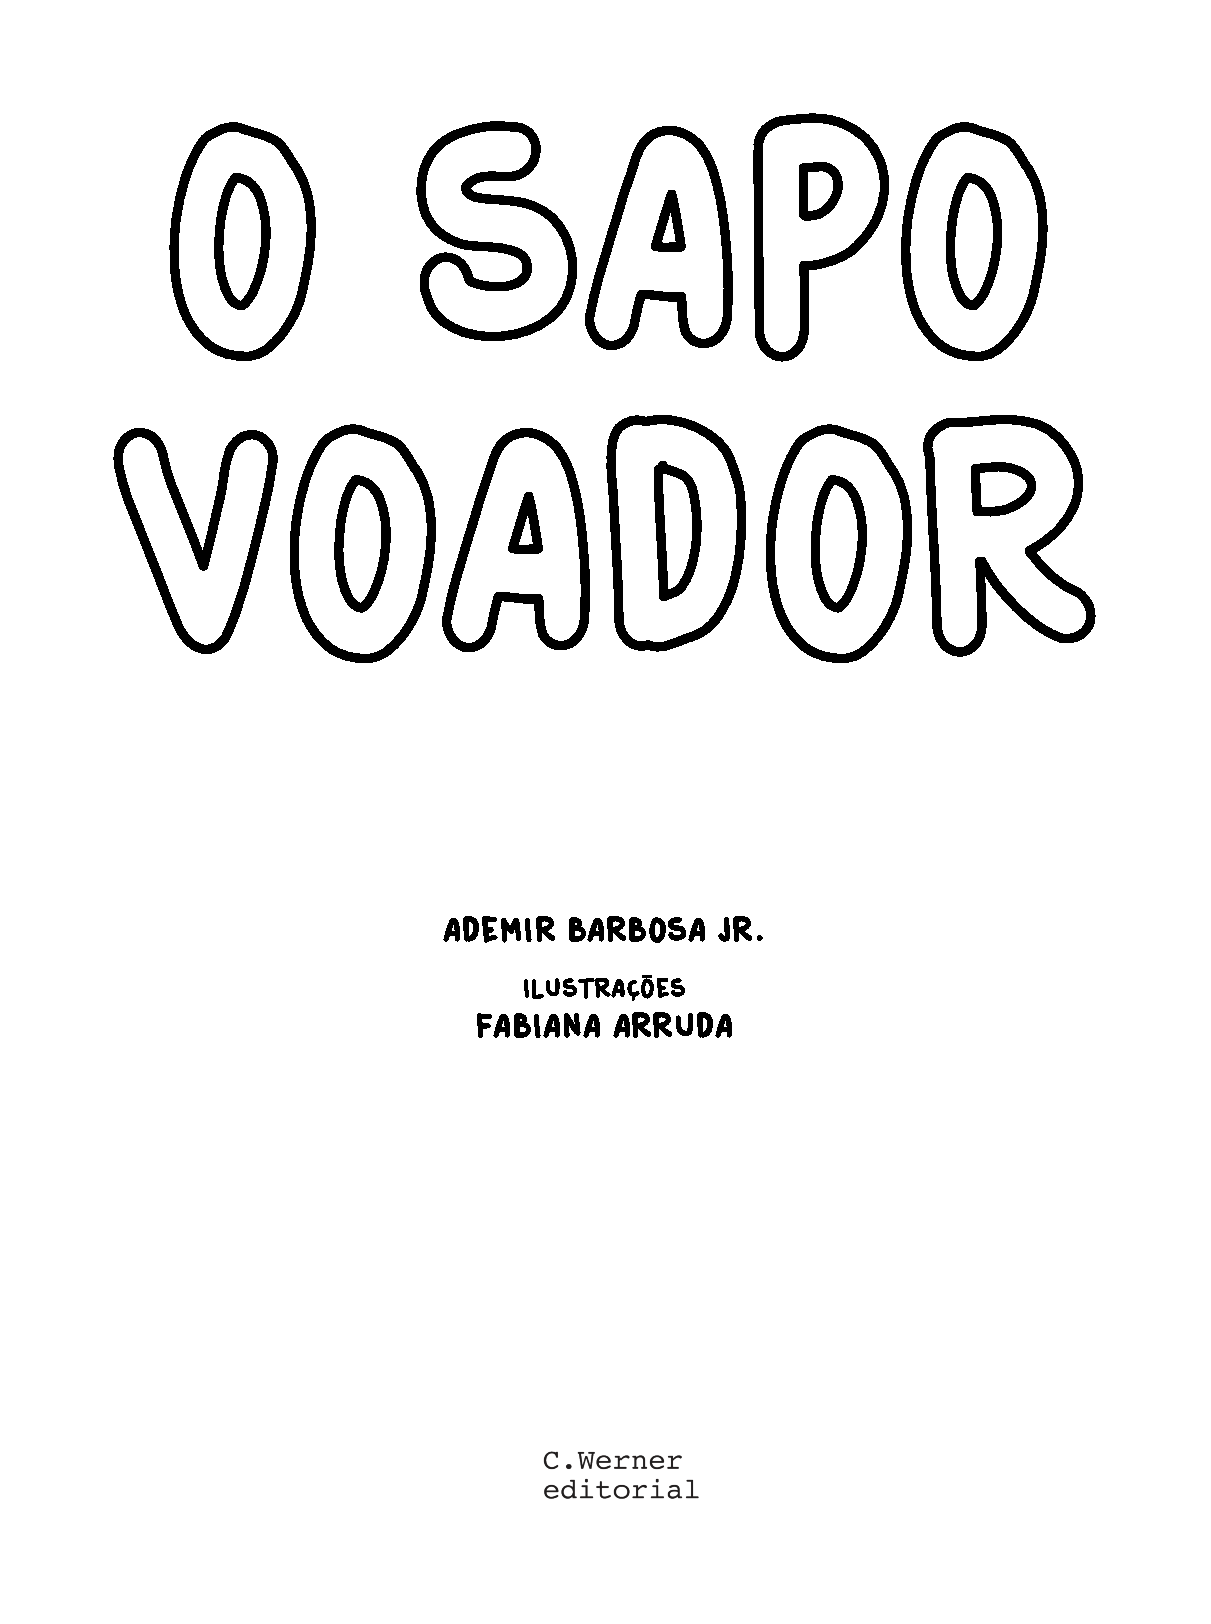
\includepdf[nup=2x2, 					% grid
			% offset=-15mm -5mm, 		% posição
			% scale=.8, 				% tamanho da página
            % delta=4mm 4mm, 			
            % frame,
            % pages={1-4}]{pdfs/PNLD2022-007_MIOLO.pdf}

\end{document}
